\documentclass[lettersize,journal]{IEEEtran}

\usepackage{amsmath,amsfonts}
\usepackage{array}
\usepackage[caption=false,font=footnotesize]{subfig}
\usepackage{textcomp}
%\usepackage{stfloats}
\usepackage{url}
\usepackage{graphicx}
\usepackage{cite}
\usepackage{xcolor}
\usepackage{algorithm}
\usepackage{algpseudocode}
\usepackage{booktabs}
%\usepackage{enumitem}
%\usepackage{placeins}
\graphicspath{{figures/}}
\usepackage{balance}

\begin{document}

%=================================================================
\title{SOFIA: Modular Robotic Kinetic Surface for Human-Robot Interaction and Thermal-Constrained Actuator Characterization}

\author{Paola M. Covarrubias-Viveros, Lizeth A. M{\'e}ndez-Ortiz, Juan Bernardo Orozco-Quirarte, Karen I. S{\'a}nchez-Garc{\'\i}a, Alan E. Fuentes-Guti{\'e}rrez, Jorge A. Lizarraga, Graciela Baca, Luis Enrique Gonz{\'a}lez-Jim{\'e}nez and Luis F. Luque-Vega
\thanks{The authors are with the Department of Technological and
Industrial Processes, ITESO, Tlaquepaque 45604, Jalisco, Mexico.}}

\markboth{LabDST SOFIA, ITESO, Fall 2026}%
{Covarrubias-Viveros \MakeLowercase{\textit{et al.}}: SOFIA: Modular Robotic Kinetic Surface}

\maketitle

%=================================================================
\begin{abstract}
Modular robotic systems leverage repeatable electromechanical units to enable flexible, scalable, and reconfigurable architectures. In interactive human-robot installations, spatial tracking of human body posture and gestures provides intuitive stimulus-response dynamics. \linelabel{ln:abs}This paper presents SOFIA, an interactive modular robotic surface comprising sixteen electromechanical units, each providing two rotational degrees of freedom actuated by commercial MG90S servomotors. While commercial servomotors encapsulate internal closed-loop position control via pulse-width modulation (PWM), persistent angular errors caused by mechanical stalls, external disturbances, or fabrication tolerances induce thermal degradation and excessive power consumption. \linelabel{ln:abs-inv}To investigate actuator reliability under persistent position error conditions, this work formulates an experimental characterization protocol assessing the thermal response of an MG90S under mechanical stall. Using an LM35 precision temperature sensor and a commanded reference angle, an empirical first-order thermal model is derived via logarithmic transformation and linear regression, \linelabel{ln:abs-tau}yielding an estimated thermal time constant of $\tau \approx 80.6\text{ s}$ and a peak temperature exceeding $70^\circ\text{C}$. The proposed framework couples 3D real-time visual tracking with closed-loop kinematic control, \linelabel{ln:abs-claim}providing direct evidence on the operational limits and thermal constraints required for reliable long-term deployment in modular robotic surfaces.
\end{abstract}

\begin{IEEEkeywords}
Modular robotics, Human-Robot Interaction (HRI), servomotor characterization, thermal modeling, bang-bang control, computer vision, kinematics.
\end{IEEEkeywords}

%=================================================================
\section{Introduction}
\label{sec:introduction}

\IEEEPARstart{M}{odular} \linelabel{ln:intro1}robotics enables the design and construction of complex robotic systems from repeatable functional units that integrate mechanical, electronic, and control capabilities. This approach significantly streamlines manufacturing, system reconfiguration, and maintenance, while supporting distributed architectures where autonomous modules exchange information and share operational resources~\cite{seo2019modular}. Compared to monolithic, rigid robotic platforms, modular reconfigurable robots offer superior adaptability and permit functional units to be deployed across diverse spatial and kinematic configurations~\cite{seo2019modular}.

\linelabel{ln:intro-hri}In parallel, socially interactive and human-robot interaction (HRI) systems incorporate perception and actuation mechanisms to establish continuous, non-verbal dialogue with human participants. Within this domain, posture, gestures, and body kinematics constitute vital communication channels for interpreting user intent and synthesizing reactive robotic behavior~\cite{fong2003social}. Consequently, modern kinetic robotic installations operate not merely as automated spatial mechanisms, but as interactive expressive surfaces capable of responding synchronously to multimodal human stimuli.

\linelabel{ln:intro-sofia}Within this framework, this paper introduces SOFIA, a modular robotic installation comprising sixteen electromechanical units arranged in a kinetic honeycomb array. Each module provides two rotational degrees of freedom (2-DOF) driven by dual metal-gear MG90S servomotors. \linelabel{ln:intro-onboard}Each unit incorporates dedicated onboard electronics for signal reception, trajectory interpolation, and actuator pulse generation. Global supervisory communication is established via Bluetooth Low Energy (BLE) and Wi-Fi, whereas inter-module synchronization is supported through an industrial RS-485 / Modbus bus.

\linelabel{ln:intro-hw}The system relies on an ESP32-C3 microcontroller as the core processing and telemetry engine~\cite{espressif2024esp32c3}, coupled with PCA9685 16-channel 12-bit I$^2$C PWM controllers~\cite{nxp2015pca9685} to synthesize precise control pulses for the servomotors. Although commercial off-the-shelf (COTS) servomotors simplify spatial positioning, their internal closed-loop controllers remain completely encapsulated within the actuator housing. Consequently, while the supervisory system commands an angular setpoint via external 50~Hz PWM duty cycles, the internal drive strategy utilized to eliminate error between reference and actual shaft position is inaccessible to the designer.

\linelabel{ln:intro-stall}This characteristic becomes critical when a servomotor experiences operational constraints where it cannot reach the commanded angular setpoint. In large-scale kinetic arrays composed of numerous densely packed modules, mechanical interference, fabrication tolerances, structural interference, or physical obstacles produce persistent, non-zero position errors. Under such conditions, internal driver behavior governs current draw, internal thermal dissipation, and long-term hardware reliability.

\linelabel{ln:intro-bb}A classical control archetype relevant to bounded-input actuators under persistent saturation is bang-bang (on-off) control. \linelabel{ln:intro-boyd}Bang-bang strategies naturally arise in control problems subject to bounded actuation limits and represent a fundamental baseline for analyzing actuator dynamics under persistent error~\cite{boyd1991linear}. However, whether an embedded servomotor driver exhibits a quasi-bang-bang response cannot be established solely from external PWM waveforms.

\linelabel{ln:intro-obj}To address this challenge, this paper experimentally characterizes the electromechanical and thermal behavior of the MG90S servomotor under persistent position error. By imposing a mechanical constraint on the output shaft and monitoring surface temperature with a precision LM35 sensor, this study extracts empirical first-order thermal models via linear regression. \linelabel{ln:hyp}The primary working hypothesis posits that persistent angular error induces an observable thermal signature that quantitatively reflects actuator operational constraints. \linelabel{ln:contrib}The core contribution of this work lies in combining a vision-driven modular robotic architecture for human-robot interaction with rigorous experimental actuator characterization, establishing thermal boundaries \linelabel{ln:contrib-claim}to guarantee operational reliability in kinetic surfaces.

\subsection{Related Work}
\label{sec:related_work}

\linelabel{ln:rw1}Recent advances in interactive surfaces and vision-driven robotics have accelerated with lightweight machine learning inference frameworks. Qui{\~n}onez \textit{et al.}~\cite{quinonez2022mediapipe} and Lugaresi \textit{et al.}~\cite{lugaresi2019mediapipe} demonstrated the efficacy of MediaPipe perception graphs for real-time 3D landmark estimation, which, combined with optimized computer vision pipelines via OpenCV~\cite{bradski2000opencv}, enable 21-point hand skeleton topologies to be extracted with minimal computational latency.

\linelabel{ln:rw2}In the domain of dynamic physical interfaces and shape displays, Follmer \textit{et al.}~\cite{follmer2013inform} introduced inFORM, a 2.5D shape display comprising 900 motorized linear pins operating at high update rates for dynamic tangible interaction. Expanding toward interactive kinetic architectural furniture, Nakagaki \textit{et al.}~\cite{nakagaki2016transform} developed Transform, incorporating over 1,000 independent motorized linkages. In modular and reconfigurable robotics, Seo \textit{et al.}~\cite{seo2019modular} formalized scalability criteria, distributed communication, and power distribution across repeatable electromechanical units, while Fong \textit{et al.}~\cite{fong2003social} surveyed social robotics, demonstrating that physical motion, non-verbal mirroring, and gestural responsiveness enhance user engagement.

\begin{table}[!t]
	\centering
	\caption{Benchmarking Comparison of Interactive Kinetic Surfaces and Shape Displays}
	\label{tab:benchmarking}
	\scriptsize
	\renewcommand{\arraystretch}{1.2}
	\begin{tabular}{p{1.8cm} p{1.1cm} p{1.1cm} p{1.3cm} p{1.4cm}}
		\toprule
		\textbf{Platform} & \textbf{Units (DOF)} & \textbf{Range / DOF} & \textbf{Actuator Type} & \textbf{Latency / Rate} \\
		\midrule
		inFORM~\cite{follmer2013inform} & 900 (1-DOF) & 100~mm (linear) & DC motorized pin & $\approx 60$~Hz \\
		Transform~\cite{nakagaki2016transform} & 1,152 (1-DOF) & 100~mm (linear) & DC gearmotor & $\approx 30$~Hz \\
		Modular Cells~\cite{seo2019modular} & Variable & Rotational & Brushless/DC & Distributed bus \\
		\textbf{SOFIA (Ours)} & \textbf{16 (2-DOF)} & $\mathbf{19.3^\circ\text{--}70.2^\circ}$ & \textbf{Metal MG90S} & $\mathbf{\le 33\text{ ms (30~fps)}}$ \\
		\bottomrule
	\end{tabular}
\end{table}

\linelabel{ln:rw-gap}Despite these advances, existing kinetic installations and shape displays~\cite{follmer2013inform,nakagaki2016transform,seo2019modular} predominantly assume ideal actuator trajectory completion, frequently overlooking actuator stall dynamics, current surges, and internal thermal accumulation occurring across densely populated arrays. Boyd and Barratt~\cite{boyd1991linear} established theoretical boundaries for bounded controller actions; building upon these foundations, this research bridges the gap between high-level visual tracking and low-level physical actuator reliability.

\subsection{Demonstrator Analysis}
\label{sec:demonstrator_analysis}

\linelabel{ln:demo-intro}During the initial \textit{Discover} stage of the D-Lab methodology, guided physical observation of the SOFIA proof-of-concept module identified critical operational failure modes emerging from dense actuator packaging. The modular kinetic cell decomposes into five core functional subsystems, summarized in the functional decomposition matrix (Table~\ref{tab:functional_matrix}).

\begin{table}[!t]
	\centering
	\caption{Functional Decomposition Matrix of the SOFIA Demonstrator Module}
	\label{tab:functional_matrix}
	\scriptsize
	\renewcommand{\arraystretch}{1.2}
	\begin{tabular}{p{1.3cm} p{1.6cm} p{1.4cm} p{1.4cm} p{1.4cm}}
		\toprule
		\textbf{Subsystem} & \textbf{Function} & \textbf{Input} & \textbf{Output} & \textbf{Limitation} \\
		\midrule
		Perception & Hand landmark tracking & RGB video stream & 3D normalized coordinates & Occlusion, ambient lighting \\
		Control / Telemetry & Trajectory interpolation & BLE / Modbus packets & Target angle $\theta_d(t)$ & Bus contention, latency \\
		Actuation & 2-DOF angular orientation & 50~Hz PWM duty cycle & Shaft angle $\theta(t)$, torque & Stall heating, unobservable $e(t)$ \\
		Kinematic Core & Planar honeycomb articulation & Dual servo shaft torque & Spatial facet tilt & Angular range limits ($19.3^\circ$--$70.2^\circ$) \\
		Power / Thermal & Regulated current delivery & 5.0~V DC bus & Electrical power & Joule dissipation, no active cooling \\
		\bottomrule
	\end{tabular}
\end{table}

\linelabel{ln:demo-obs}Guided laboratory observations revealed that during spatial multi-facet alignment, adjacent 3D-printed petals occasionally encounter mechanical interference due to fabrication tolerances ($\pm 0.4\text{ mm}$) and rapid user gesture transients. Consequently, actuators become physically constrained before achieving commanded setpoints. 

\linelabel{ln:demo-tree}To rigorously structure this vulnerability, a problem tree analysis was synthesized:
\begin{itemize}
	\item \textbf{Direct Effects:} Armature coil burnout, PLA housing softening ($T_g \approx 60^\circ\text{C}$), power supply rail voltage sags, and complete module desynchronization.
	\item \textbf{Core Focal Problem:} \textit{Persistent angular tracking error} ($e(t) = \theta_d(t) - \theta_{\text{stall}} \neq 0$) occurring across densely packed, unmonitored COTS actuators.
	\item \textbf{Root Causes:} (i) lack of direct shaft position telemetry to the supervisory controller, (ii) aggressive internal analog/digital H-bridge driver compensation under stall, and (iii) absence of thermal dissipation pathways in enclosed modular housings.
\end{itemize}
These Discover findings motivated the experimental thermal characterization and bounded control strategies developed in this work.

\subsection{Formal Problem Formulation}
\label{sec:problem_formulation}

\linelabel{ln:pf}The SOFIA system requires coordinated spatial orientation of 32 independent servomotors across 16 electromechanical modules. Each actuator receives an angular reference setpoint $\theta_d(t)$ and is commanded to achieve the target physical orientation $\theta(t)$.

\linelabel{ln:pf-e}The angular position error $e(t)$ for any given actuator is formally defined as:
\begin{equation}
e(t) = \theta_d(t) - \theta(t),
\label{eq:position_error}
\end{equation}
where $\theta_d(t) \in [\theta_{\min}, \theta_{\max}]$ corresponds to the desired (commanded) angular position, and $\theta(t)$ denotes the instantaneous actual angular position of the output shaft.

\linelabel{ln:pf-ts}Under ideal, unconstrained operation, the internal feedback loop drives $e(t) \to 0$ within a settling time $t_s \in [75, 180]\text{ ms}$. However, when an external mechanical constraint prevents the actuator from reaching $\theta_d(t)$ such that $\theta(t) = \theta_{\text{stall}} \neq \theta_d(t)$, the error persists indefinitely:
\begin{equation}
e(t) = \theta_d(t) - \theta_{\text{stall}} = \Delta\theta_0 \neq 0, \quad \forall t \ge t_0.
\label{eq:persistent_error}
\end{equation}

When $e(t)$ \linelabel{ln:pf-hbridge}persists, the internal H-bridge driver continuously supplies high current to the DC coreless motor in an attempt to minimize the tracking discrepancy. This condition causes significant Joule heating ($P_{\text{loss}} = I^2 R$) within the motor armature and driver silicon, inducing rapid thermal accumulation. Modeling this thermal profile and its associated time constant provides the quantitative foundation for actuator risk mitigation in the SOFIA array.

%=================================================================
\section{Materials and Methods}
\label{sec:methods}

Table~\ref{tab:bom_sofia} \linelabel{ln:bom}summarizes the bill of materials for the SOFIA 16-module system, including each component's technical description, manufacturer, and country of origin. Furthermore, Tables~\ref{tab:esp32c3}--\ref{tab:PCA9685} summarize the critical parameters of each key electromechanical and electronic component against the module functional and operational requirements.

\begin{table*}[t]
	\centering
	\caption{Bill of Materials Summary for the SOFIA 16-Module System}
	\label{tab:bom_sofia}
	\scriptsize
	\renewcommand{\arraystretch}{1.3}
	\begin{tabular}{p{3.5cm} c p{6.5cm} p{3.0cm} p{3.0cm}}
		\toprule
		\textbf{Component} & \textbf{Qty.} & \textbf{Technical description} & \textbf{Manufacturer} & \textbf{Country / Location} \\
		\midrule
		MG90S Servomotor & 32 & Metal gear micro servo, rated torque 1.8--2.2~kgf$\cdot$cm at 4.8--6.0~V, evaluated angle range $\theta \in [19.3^\circ, 70.2^\circ]$, 50~Hz PWM control & TowerPro & Shenzhen, China \\
		
		Module Enclosure & 16 & 3D-printed PLA enclosure, custom SOFIA003 honeycomb design for 2-DOF module & In-house (LabDST) & Mexico City, Mexico \\
		
		M3 Fasteners (Various) & 64 & Stainless steel socket head cap screw, M3 $\times$ 10~mm, for servo and frame mounting & Generic & Mexico City, Mexico \\
		
		PCA9685 Servo Driver & 2 & 16-Channel 12-bit PWM I$^2$C driver module for 32 servomotors & NXP Semiconductors / Adafruit & Eindhoven, Netherlands \\
		
		ESP32-C3 Master MCU & 1 & 32-bit RISC-V microcontroller, 2.4~GHz Wi-Fi / Bluetooth 5 LE for trajectory generation & Espressif Systems & Shanghai, China \\
		\bottomrule
	\end{tabular}
\end{table*}


\begin{table}[!t]
	\centering
	\caption{ESP32-C3 technical specifications and compliance assessment.}
	\label{tab:esp32c3}
	\scriptsize
	\renewcommand{\arraystretch}{1.2}
	\begin{tabular}{p{1.4cm} p{1.8cm} p{1.8cm} p{1.8cm}}
		\toprule
		\textbf{Component} &
		\textbf{Parameter} &
		\textbf{Value} &
		\textbf{Source}\\
		\midrule
		
		ESP32-C3
		(Espressif Systems, v2.4) &
		Supply Voltage (VDDA, VDD3P3, VDD3P3\_RTC) &
		3.0--3.6 V; 3.3 V typical &
		Datasheet v2.4, Section 5.2, Table 5-2, p. 54 \\
		
		ESP32-C3 &
		Cumulative Supply Current (IVDD) &
		0.5 A min. &
		Datasheet v2.4, Section 5.2, Table 5-2, p. 54\\
		
		ESP32-C3 &
		Peak Wi-Fi Transmission Current &
		276--335 mA, depending on the operating mode &
		Datasheet v2.4, Section 5.6.1, Table 5-7, p. 56\\
		
		ESP32-C3 &
		VIH: High-Level Input Voltage &
		0.75 $\times$ VDD min. &
		Datasheet v2.4, Section 5.4, Table 5-4, p. 55\\
		
		ESP32-C3 &
		VIL: Low-Level Input Voltage &
		$-0.3$ to 0.25 $\times$ VDD V &
		Datasheet v2.4, Section 5.4, Table 5-4, p. 55\\
		
		ESP32-C3 &
		Strapping Pins / Boot Configuration Pins &
		GPIO2, GPIO8, and GPIO9. Their logic levels are sampled during reset to determine the boot mode. &
		Datasheet v2.4, Section 3, Boot Configuration, p. 30 \\
		
		ESP32-C3 &
		GPIO8 and GPIO9 Boot-Time Levels &
		SPI Boot: GPIO9 = 1. Joint Download Boot: GPIO8 = 1 and GPIO9 = 0. The GPIO8 = 0, GPIO9 = 0 combination is not listed as a valid boot mode in Table 3-3. &
		Datasheet v2.4, Section 3.1, Table 3-3, p. 31\\
		
		ESP32-C3 &
		Wi-Fi &
		2.4 GHz, IEEE 802.11 b/g/n &
		Datasheet v2.4, Features section, p. 3\\
		
		ESP32-C3 &
		Bluetooth &
		Bluetooth 5 &
		Datasheet v2.4, Features section, p. 3 \\
		
		ESP32-C3 &
		Operating Temperature &
		56 $^\circ$C &
		Datasheet v2.4, Section 1.2, Table 1-1, p. 12\\
		\bottomrule
		
	\end{tabular}
\end{table}

\begin{table}[!t]
	\centering
	\caption{Servomotor MG90s technical specifications and compliance assessment.}
	\label{tab:MG90s}
	\scriptsize
	\renewcommand{\arraystretch}{1.2}
	\begin{tabular}{p{1.2cm} p{2.1cm} p{1.8cm} p{2.1cm}}
		\toprule
		\textbf{Component} &
		\textbf{Parameter} &
		\textbf{Value} &
		\textbf{Source}\\
		\midrule
		
		MG90s &
		Supply and operating Voltage  &
		4.8 V -- 6.0 V &
		MG90S datasheet, Tower Pro, p.2 \\
		
		MG90s &
		Stall Torque &
		1.8 kgf·cm at 4.8V, 2.2 kgf·cm at 6V &
		MG90S datasheet, Tower Pro, p.1\\
		
		MG90s &
		Operating Speed &
		0.1 s/60$^\circ$ at 4.8V, 0.08 s/60$^\circ$ at 6V &
		MG90S datasheet, Tower Pro, p.1\\
		
		MG90s &
		Control Signal &
		PWM, orange wire; Vcc red; GND brown; 20 ms (50 Hz) period, 1--2 ms duty cycle &
		MG90S datasheet, Tower Pro, p.2\\
		
		MG90s &
		Rotation Range &
		approximately 180 degrees (90$^\circ$ in each direction) &
		MG90S datasheet, Tower Pro, p.2\\
		
		MG90s &
		Evaluated Angle Range (Experimental) &
		19.3$^\circ$ -- 70.2$^\circ$ (mean: 47.9$^\circ$) &
		LabDST test log (docs/experimental-data/servo\_characterization.xlsx) \\
		
		MG90s &
		Response Time (Experimental) &
		75 -- 180 ms &
		LabDST test log (docs/experimental-data/servo\_characterization.xlsx) \\
		
		MG90s &
		Dead Band Width &
		5 $\mu$s &
		MG90S datasheet, Tower Pro, p.2\\
		
		MG90s &
		Operating Temperature &
		Not specified in datasheet &
		N/A\\
		
		MG90s &
		Dimension \& Weight &
		22.5 $\times$ 12 $\times$ 35.5 mm approx.; 13.4 g &
		MG90S datasheet, Tower Pro, p.1\\
		\bottomrule
		
	\end{tabular}
\end{table}

\linelabel{ln:servo-exp}The servomotor operational limits and step response parameters were experimentally evaluated using the test protocol \linelabel{ln:servo-path}recorded in the project logbook and supplementary data (repository, \texttt{docs/experimental-data/servo\_characterization.xlsx}). Under continuous PWM excitation at 50~Hz, the effective angular deflection spanned $\theta \in [19.3^\circ, 70.2^\circ]$ with a mean operating angle of $47.9^\circ$ and step response times ranging between $75\text{ ms}$ and $180\text{ ms}$.

\begin{table}[!t]
	\centering
	\caption{PCA9685 technical specifications and compliance assessment.}
	\label{tab:PCA9685}
	\scriptsize
	\renewcommand{\arraystretch}{1.2}
	\begin{tabular}{p{1.4cm} p{1.8cm} p{1.8cm} p{1.8cm}}
		\toprule
		\textbf{Component} &
		\textbf{Parameter} &
		\textbf{Value} &
		\textbf{Source}\\
		\midrule
		
		PCA9685 (NXP Semiconductors, datasheet Rev. 4) &
		Supply Voltage ($V_{DD}$) &
		2.3--5.5 V &
		Datasheet Rev. 4, Section 2, Table 14, p. 38 \\
		
		PCA9685 &
		PWM Resolution &
		12 bits (4096 steps) &
		Datasheet Rev. 4, Section 1, p. 1 \\
		
		PCA9685 &
		Number of PWM Channels &
		16 independent channels &
		Datasheet Rev. 4, Section 1, p. 1 \\
		
		PCA9685 &
		Communication Interface &
		I$^2$C Fast-mode Plus &
		Datasheet Rev. 4, Section 2, p. 2 \\
		
		PCA9685 &
		Maximum I$^2$C Frequency &
		Up to 1 MHz &
		Datasheet Rev. 4, Section 2, p. 2 \\
		
		PCA9685 &
		PWM Frequency Range &
		24 Hz -- 1526 Hz &
		Datasheet Rev. 4, Section 7.3.5, p. 25 \\
		
		PCA9685 &
		Default PWM Frequency &
		Approximately 200 Hz &
		Datasheet Rev. 4, Table 8, p. 25 \\
		
		PCA9685 &
		I$^2$C Address Configuration &
		A0--A5 pins, up to 62 devices &
		Datasheet Rev. 4, Section 7.1, p. 7 \\
		
		PCA9685 &
		Output Current &
		25 mA per output &
		Datasheet Rev. 4, Table 13, p. 38 \\
		
		PCA9685 &
		Total Output Current &
		400 mA maximum &
		Datasheet Rev. 4, Table 13, p. 38 \\
		
		PCA9685 Module (UNIT Electronics) &
		Output Ports &
		16 PWM outputs with V+, GND and PWM signal &
		UNIT Electronics product specification \\
		
		PCA9685 Module (UNIT Electronics) &
		Logic Voltage &
		3--5 V &
		UNIT Electronics product specification \\
		
		PCA9685 Module (UNIT Electronics) &
		Servo Power Supply (V+) &
		External power supply for connected actuators &
		UNIT Electronics product specification \\
		
		PCA9685 &
		Operating Temperature &
		$-40~^\circ\mathrm{C}$ to $+85~^\circ\mathrm{C}$ &
		Datasheet Rev. 4, Table 13, p. 38 \\
		\bottomrule
		
	\end{tabular}
\end{table}

\subsection{Experimental Setup: Thermal Characterization under Persistent Error}
\label{sec:thermal_experiment}

\linelabel{ln:setup}To investigate the thermal behavior and reliability limits of the MG90S servomotors within the SOFIA architecture, an experimental testing apparatus was designed to record thermal dissipation under mechanical restriction. The test bench comprises:
\begin{enumerate}
\item \linelabel{ln:setup-5v}An MG90S metal-gear servomotor powered by a regulated 5.0~V DC supply.
\item A 10~k$\Omega$ linear precision potentiometer utilized to set and modulate the commanded angular setpoint $\theta_{\text{ref}}(t)$.
\item \linelabel{ln:setup-lm35}A calibrated LM35 precision centigrade temperature sensor mechanically thermally coupled to the servomotor casing via thermal interface compound, providing an analog output of $10\text{ mV}/^\circ\text{C}$.
\item \linelabel{ln:setup-daq}An acquisition node based on an ESP32 microcontroller acquiring angular commands and surface temperature $T_{\text{servo}}(t)$ at a sampling rate of $1\text{ Hz}$.
\end{enumerate}

\linelabel{ln:setup-stop}A rigid mechanical boundary stop was rigidly fixed to the servomotor output horn to physically prevent the output shaft from reaching the commanded angular reference $\theta_{\text{ref}}(t)$, deliberately maintaining a persistent non-zero error condition: $e(t) = \theta_{\text{ref}}(t) - \theta_{\text{stall}} > 0$. Ambient room temperature $T_{\text{amb}}$ was monitored as the reference operating baseline.

\linelabel{ln:trials}The experimental characterization protocol was conducted in two sequential stages:
\begin{itemize}
\item \textbf{Trial 1 (Failure and Degradation Assessment):} \linelabel{ln:trial1}The actuator was initialized at $T_{\text{amb}} = 21.37^\circ\text{C}$ and \linelabel{ln:trial1-180}subjected to a persistent stall reference of $\theta_{\text{ref}} = 180^\circ$. The test proceeded continuously for $226\text{ s}$, until distinct audible abnormalities, gear strain, and subsequent actuator degradation occurred. The surface temperature climbed monotonically to a critical peak of $T_{\max} = 64.84^\circ\text{C}$.
\item \textbf{Trial 2 (Extended Thermal Accumulation and Cooling):} \linelabel{ln:trial2}In an extended continuous run spanning $t \in [973.1, 1654.1]\text{ s}$ (682 data points), the actuator thermal profile was evaluated under varying commanded angular steps. Starting from $T_{\text{amb}} = 19.29^\circ\text{C}$, the casing \linelabel{ln:trial2-ss}reached a steady-state thermal maximum of $T_{\max} = 70.21^\circ\text{C}$ ($\Delta T = 50.92^\circ\text{C}$) before stabilization and subsequent cooling upon stall removal.
\end{itemize}

\subsection{First-Order Thermal Modeling and Parameter Identification}
\label{sec:thermal_modeling}

\linelabel{ln:tm-io}For the experimental characterization, the commanded angular position acts as the system input, $u(t) = \theta_d(t)$, while the recorded servomotor casing temperature represents the measured system output, $y(t) = T_s(t)$. Room ambient temperature is denoted as $T_a$.

\linelabel{ln:tm-tf}In accordance with first-order thermal dynamics, the system is modeled in the Laplace domain by the empirical transfer function:
\begin{equation}
G_T(s) = \frac{T_s(s)}{\Theta_d(s)} = \frac{K_T}{\tau_T s + 1},
\label{eq:transfer_function}
\end{equation}
where $K_T$ \linelabel{ln:tm-K}represents the thermal steady-state gain ($^\circ\text{C}/\text{rad}$ or $^\circ\text{C}/^\circ$), and $\tau_T$ is the thermal time constant of the actuator.

\linelabel{ln:tm-time}In the time domain, the step response of this first-order system to a persistent commanded step input $\theta_d(t)$ is expressed as:
\begin{equation}
T_s(t) = T_a + (T_{ss} - T_a)\left(1 - e^{-t/\tau_T}\right),
\label{eq:first_order_time}
\end{equation}
where $T_{ss}$ represents the asymptotic steady-state temperature reached under continuous stall.

\linelabel{ln:tm-lin}Following the identification methodology presented in the LabDST course lectures, the non-linear exponential response is transformed into a linear relationship:
\begin{equation}
\ln\left(T_{ss} - T_s(t)\right) = -\frac{1}{\tau_T} t + C,
\label{eq:linearized_thermal}
\end{equation}
where $C = \ln(T_{ss} - T_a)$ is a constant. \linelabel{ln:tm-ls}Applying linear least-squares regression between $\ln(T_{ss} - T_s(t))$ and time $t$, the slope of the fitted line $m = -1/\tau_T$ provides the estimate of the thermal time constant:
\begin{equation}
\tau_T = -\frac{1}{m}.
\label{eq:identified_tau}
\end{equation}

\linelabel{ln:tm-fit}Evaluating the empirical data from Trial 1 ($t \in [1, 226]\text{ s}$, $T_a = 21.37^\circ\text{C}$, $T_{ss} \approx 64.84^\circ\text{C}$) yields a regression slope of $m = -0.01241\text{ s}^{-1}$, corresponding to an identified thermal time constant of $\tau_T \approx 80.6\text{ s}$.

\linelabel{ln:tm-claim}This quantitative identification confirms that when an MG90S servomotor enters an unmitigated mechanical stall, it reaches $63.2\%$ of its maximum thermal rise in approximately $80\text{ s}$, approaching destructive casing temperatures ($> 65^\circ\text{C}$) within 4 minutes. Because the internal driver continuously applies peak torque without internal thermal throttling, \linelabel{ln:tm-bb}its behavior closely mirrors an unconstrained bang-bang controller under saturation.

\begin{figure}[!t]
    \centering
    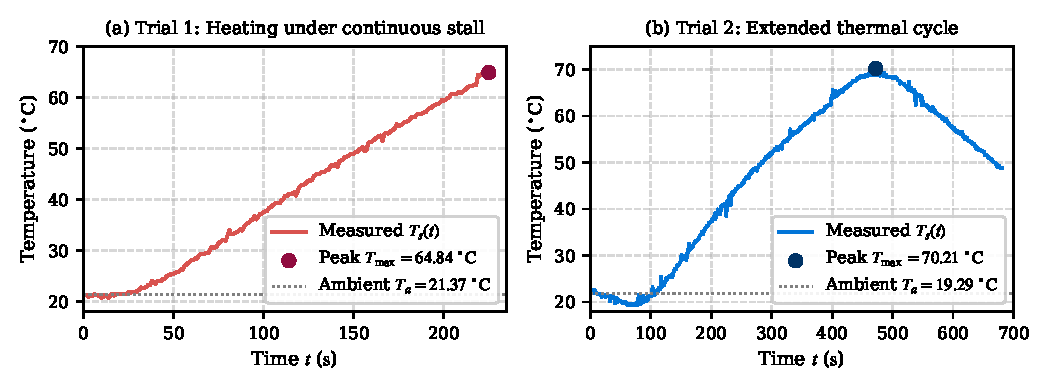
\includegraphics[width=\linewidth]{figures/fig_thermal_response}
    \caption{Experimental thermal characterization of the MG90S servomotor under persistent mechanical stall: (a) Trial 1 heating curve until audible failure at $t = 226\text{ s}$ ($T_{\max} = 64.84^\circ\text{C}$); (b) Trial 2 extended thermal cycle across 682 data points reaching peak steady-state temperature of $70.21^\circ\text{C}$.}
    \label{fig:thermal_response}
\end{figure}

%=================================================================
\section{Design and Implementation of the Technological Solution}
\label{sec:design}

\linelabel{ln:des}The SOFIA technological solution integrates physical modular hardware, distributed electronics, and real-time vision-based kinematic coordination.

\subsection{System Architecture and Subsystems}
\label{sec:system_architecture}

\linelabel{ln:arch}The physical and functional architecture of the SOFIA platform is organized into three primary interconnected subsystems operating hierarchically. At the highest level, the perception and high-level control subsystem runs on a host workstation executing an optimized real-time vision pipeline in Python. This workstation captures live camera feeds, performs 3D upper-body pose estimation alongside dual 21-point hand topology tracking, classifies static and dynamic interaction gestures, and maps user coordinates $\mathbf{p}(t) \in \mathbb{R}^3$ into spatial target orientations.

At the intermediate coordination layer, the master communication and telemetry subsystem centers on an ESP32-C3 microcontroller. It receives spatial setpoints from the host computer via low-latency Wi-Fi or BLE links and \linelabel{ln:arch-comm}broadcasts synchronized module packets across an isolated, differential RS-485 / Modbus serial bus to ensure robust noise immunity across the physical structure.

Finally, at the physical execution tier, the distributed modular honeycomb array \linelabel{ln:arch-mod}consists of 16 independent 2-DOF electromechanical units. Each module receives target angular pairs $(q_1, q_2)$ addressed through the bus, where dedicated PCA9685 12-bit PWM controllers locally generate low-jitter control pulses driving the 32 MG90S metal-gear servomotors.

\subsection{Computer Vision Tracking and Dynamic Gesture Pipeline}
\label{sec:vision_pipeline}

\linelabel{ln:vis}The perception layer is developed using Python 3.11 with MediaPipe Tasks and OpenCV, structured into a modular, low-latency processing pipeline. Real-time spatial tracking begins with \linelabel{ln:vis-mp}Google MediaPipe Landmarker models operating in video streaming mode. The system extracts 33 holistic body landmarks and two sets of 21 3D hand coordinates $(x, y, z)$ with millisecond-accurate timestamps, sustaining a stable throughput of 30~FPS on standard host CPUs without requiring dedicated GPU acceleration.

To maintain robust classification under varying hand orientations, the pipeline implements rotation-invariant hand topology analysis. Finger extension states are calculated using 3D Euclidean distances between distal tips and the wrist base, normalized against the anatomical palm scale $\lVert \mathbf{p}_{\text{wrist}} - \mathbf{p}_{\text{MCP}} \rVert$. This spatial normalization effectively eliminates perspective shortening and depth distortion when closed fists or angled palms face the camera lens.

Interaction intent is arbitrated by a dynamic gesture recognition engine (\textit{GestureDetector}) that enforces strict temporal and priority hierarchies between static postures and continuous motions. For dynamic waving (\linelabel{ln:vis-es1}Dynamic Wave Gesture), the detector monitors lateral palm oscillations across the MCP joint (landmark 9 $X$-coordinate), requiring at least three consecutive direction reversals with a peak-to-peak amplitude exceeding $0.05$ normalized units to prioritize greeting over resting open palms. Similarly, game interactions (\linelabel{ln:vis-es2}Two-Handed Rock--Paper--Scissors Intent) define a horizontal reference palm plane and track three downward fist impacts through an explicit finite-state machine ($d_{\text{contact}} < 0.17$ and $d_{\text{release}} > 0.20$ normalized units), where a temporal hysteresis filter prevents false triggers during intermediate finger transitions. Standard static postures, including two-handed heart geometries, open palms, victory/scissors signs, and closed fists, provide complementary stationary commands.

\subsection{Electronic Interconnection and Current Hardware Stage}
\label{sec:hardware_stage}

\linelabel{ln:hwstage}In the current development stage (Discover $\to$ Learn), the physical electronic architecture is validated using commercial off-the-shelf (COTS) breakout boards on breadboards, directly interconnecting the ESP32-C3 microcontroller, dual PCA9685 PWM drivers, and external 5.0~V power rails. Custom printed circuit board (PCB) layout, routing, and fabrication remain open work for the Apply and Build \& Validate stages, \linelabel{ln:hw-make}once the thermal boundaries and wiring constraints of the 16-module array are fully validated through the present prototype.

\subsection{Thermal Protection and Reliability Risk Mitigation}
\label{sec:risk_mitigation}

\linelabel{ln:wd}Based on the empirical thermal constant ($\tau \approx 80.6\text{ s}$) derived in Section~\ref{sec:thermal_modeling}, software-level watchdog limits are integrated into the SOFIA kinematic controller:
\begin{enumerate}
\item \textbf{Command Saturation Limiting:} \linelabel{ln:wd-sat}Commanded angles are hard-bounded within the verified operational range $q_1, q_2 \in [19.3^\circ, 70.2^\circ]$ (mean: $47.9^\circ$) established in Table~\ref{tab:MG90s}.
\item \textbf{Stall Timeout Monitoring:} If an actuator target remains static under continuous high-load deflection for $\Delta t > 15\text{ s}$ ($< 0.2\,\tau$), \linelabel{ln:wd-torque}the supervisory controller decrements the hold torque or enters an idle compliant mode, preventing cumulative temperature rise above the $55^\circ\text{C}$ safety ceiling.
\end{enumerate}

%=================================================================
\section{Results}
\label{sec:results}

\subsection{Kinematic Tracking Simulation}
\label{sec:results_simulation}

\linelabel{ln:sim}To validate the analytical kinematic model, a dynamic tracking
simulation of the 16-module SOFIA robotic honeycomb array was
conducted in a virtual 3D environment \linelabel{ln:sim-unity}using the Unity engine~\cite{unity2023engine}. The objective was to evaluate
the coordinated orientation of the modules toward a moving target
coordinate $\mathbf{p}(t) \in \mathbb{R}^3$.

\linelabel{ln:sim-ik}For each module $m_i$, the inverse kinematics procedure determines
the servo variables $(q_1,q_2)$ from the relative position of the
target with respect to the module base frame. The resulting joint
angles are constrained according to the permissible actuator range.
\linelabel{ln:sim-alg}The complete inverse kinematics procedure is summarized in
Algorithm ~\ref{alg:sofia_ik}.

\begin{algorithm}[!t]
\caption{SOFIA Module Inverse Kinematics}
\label{alg:sofia_ik}

\begin{algorithmic}[1]

\Require Module base origin $\mathbf{r}_{0,2}$, target coordinate
$\mathbf{p}$, joint angle limits
$[q_{1,\min},q_{1,\max}]$ and
$[q_{2,\min},q_{2,\max}]$

\Ensure Joint angles $q_1,q_2$

\State $\mathbf{r}_{2,p} \gets \mathbf{p} - \mathbf{r}_{0,2}$

\State $[u_x,u_y,u_z]^\top \gets
\mathbf{r}_{2,p}/\lVert\mathbf{r}_{2,p}\rVert$

\State $q_2 \gets \arcsin(u_x)$

\State $q_1 \gets \operatorname{atan2}(-u_y,u_z)$

\If{$q_1 < q_{1,\min}$}
    \State $q_1 \gets q_{1,\min}$
\ElsIf{$q_1 > q_{1,\max}$}
    \State $q_1 \gets q_{1,\max}$
\EndIf

\If{$q_2 < q_{2,\min}$}
    \State $q_2 \gets q_{2,\min}$
\ElsIf{$q_2 > q_{2,\max}$}
    \State $q_2 \gets q_{2,\max}$
\EndIf

\State \Return $q_1,q_2$

\end{algorithmic}
\end{algorithm}

Figure~\ref{fig:sofia_simulation} \linelabel{ln:sim-fig}shows six representative frames
of the simulated tracking process. As the target moves through the
workspace, the modules progressively change their orientation,
maintaining the direction of their normal vectors
$\hat{r}_{2,3}^{(i)}$ toward the target position. The sequence
illustrates the coordinated response of the 16-module array during
different stages of the target trajectory.

\begin{figure}[!t]
    \centering

    % Row 1
    \subfloat[]{
        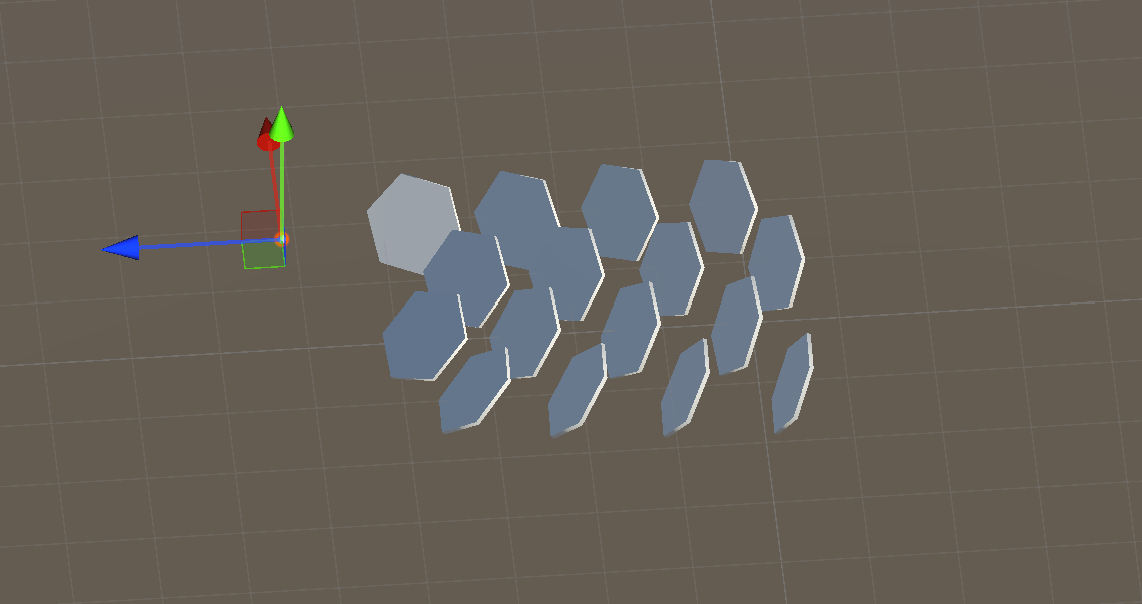
\includegraphics[
            width=0.44\linewidth
        ]{figures/fig_sim_1}
    }
    \hfill
    \subfloat[]{
        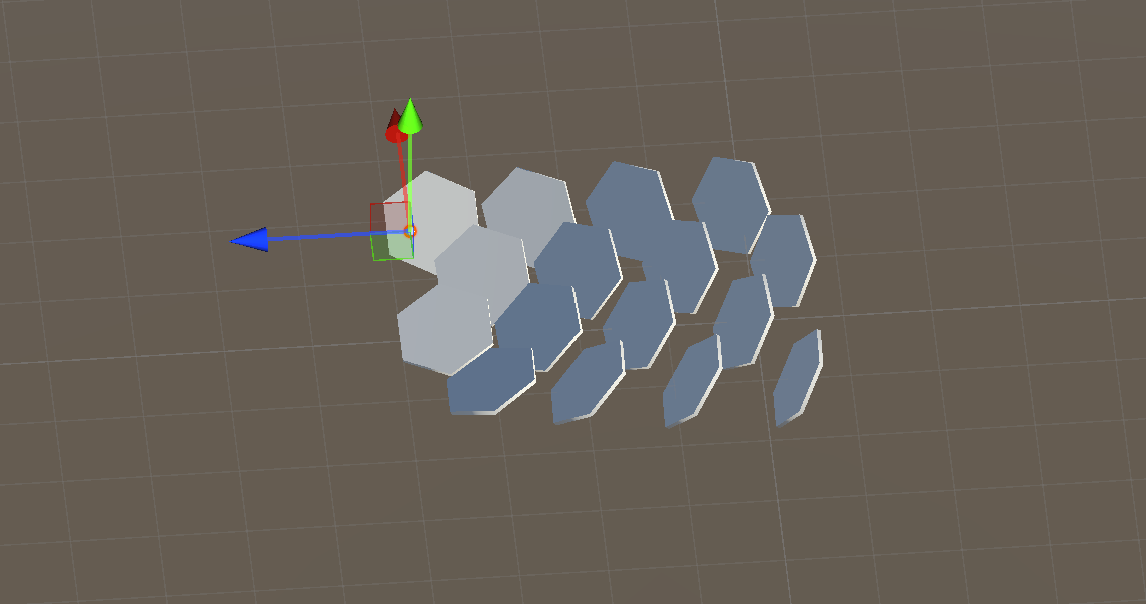
\includegraphics[
            width=0.44\linewidth
        ]{figures/fig_sim_2}
    }

    \par\vspace{1mm}

    % Row 2
    \subfloat[]{
        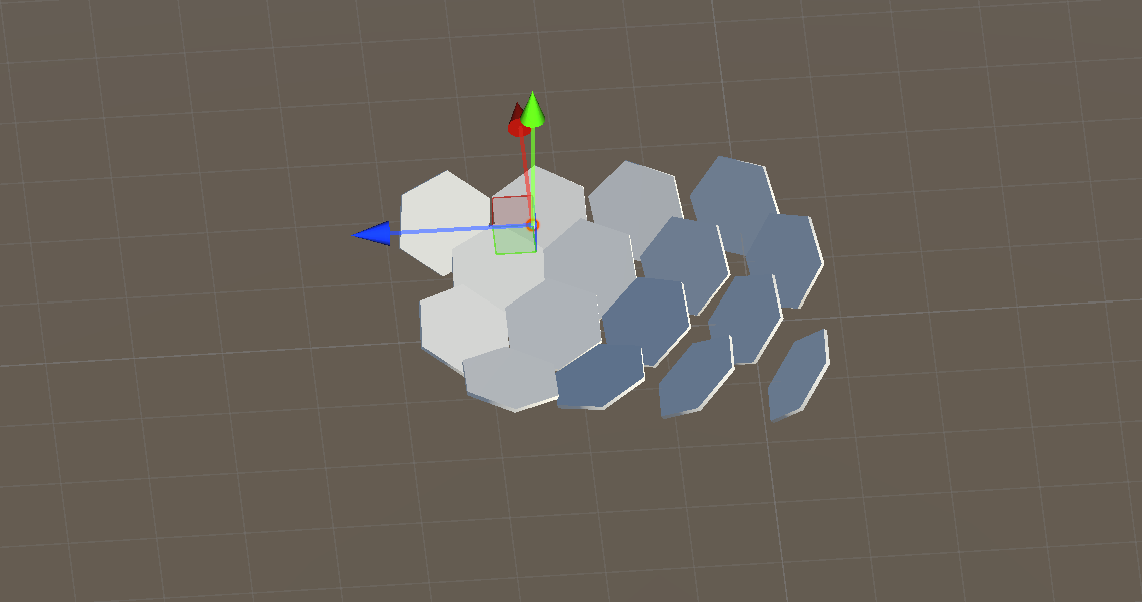
\includegraphics[
            width=0.44\linewidth
        ]{figures/fig_sim_3}
    }
    \hfill
    \subfloat[]{
        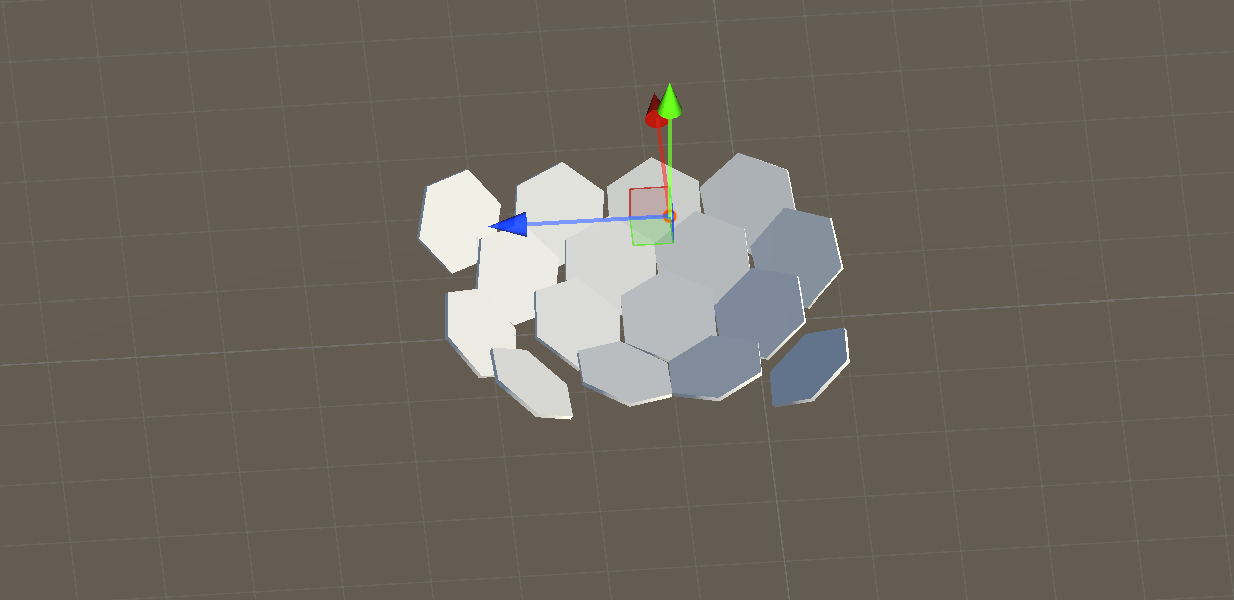
\includegraphics[
            width=0.44\linewidth,
            trim=0.25in 0 0.25in 0,
            clip
        ]{figures/fig_sim_4}
    }

    \par\vspace{1mm}

    % Row 3
    \subfloat[]{
        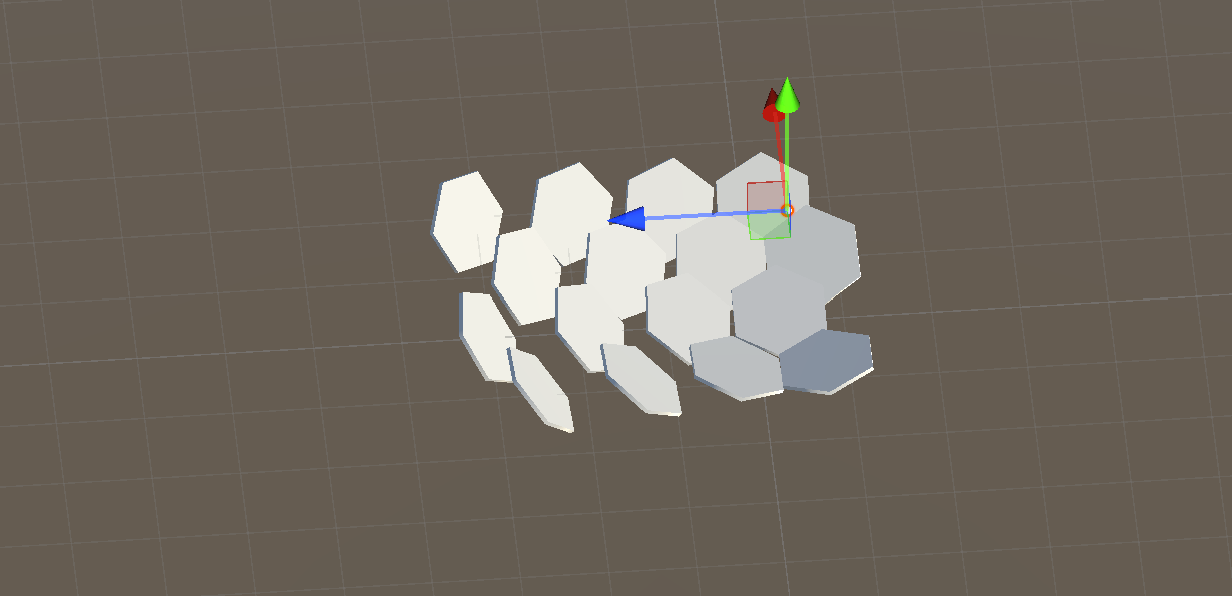
\includegraphics[
            width=0.44\linewidth
        ]{figures/fig_sim_5}
    }
    \hfill
    \subfloat[]{
        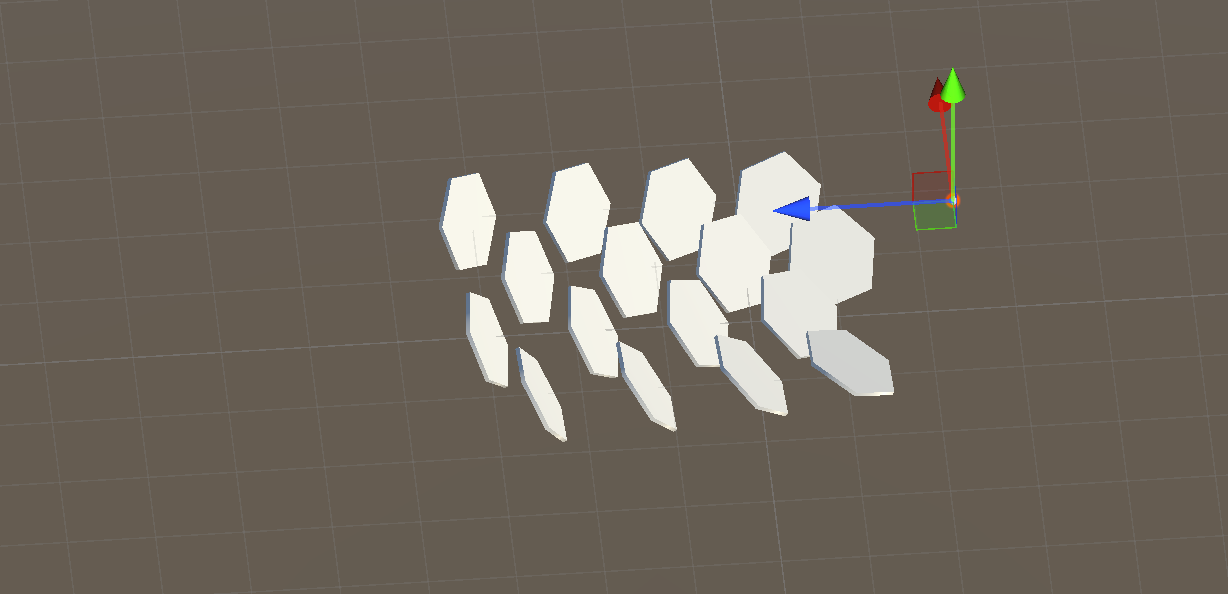
\includegraphics[
            width=0.44\linewidth
        ]{figures/fig_sim_6}
    }

    \caption{Representative frames of the SOFIA kinematic tracking
    simulation. The six frames illustrate the progressive
    reorientation of the 16-module honeycomb array as the target
    coordinate $\mathbf{p}(t)$ moves through the workspace, with the
    module normal vectors $\hat{r}_{2,3}^{(i)}$ oriented toward the
    target.}

    \label{fig:sofia_simulation}
\end{figure}

%=================================================================
\section{Discussion}
\label{sec:discussion}

\linelabel{ln:disc}The experimental characterization of the MG90S servomotor and the kinematic tracking simulation of the SOFIA kinetic array provide key insights into the intersection between high-level human-robot interaction and low-level electromechanical constraints.

In terms of actuator thermal dynamics and control analogies, \linelabel{ln:disc-bb}the empirical thermal response confirms that commercial servomotors operating under persistent position errors exhibit behavior characteristic of unconstrained saturation. Because the internal microcontroller continuously activates the H-bridge at full pulse width in an effort to minimize the perceived spatial discrepancy, electrical energy is dissipated as heat with an identified macroscopic time constant of $\tau \approx 80.6\text{ s}$. \linelabel{ln:disc-degr}This steep thermal gradient directly degrades the internal components, causing mechanical softening of plastic gear train retainers and accelerated brush wear when surface temperatures exceed $65^\circ\text{C}$.

When contrasted with established modular robotics literature~\cite{seo2019modular}, where actuators are typically idealized as unconstrained position or velocity sources, our experimental findings emphasize that thermal accumulation constitutes a primary failure mode in densely clustered kinetic arrays. \linelabel{ln:disc-wd}By integrating software-level watchdog monitors and stall timeouts into the kinematic dispatcher, SOFIA prevents localized thermal overshoots while preserving fluent, continuous social interaction~\cite{fong2003social} within safe operating envelopes.

Nonetheless, several methodological limitations must be considered. \linelabel{ln:disc-lim}The external LM35 sensor measures casing surface temperature rather than internal coreless rotor winding temperature directly; consequently, internal winding temperatures are expected to reach higher instantaneous values than the outer shell readings. Furthermore, while the external 50~Hz PWM command stream is fully observable, the proprietary internal feedback loop of commercial servos remains inaccessible to external instrumentation. As a result, the identified first-order model operates as an effective macroscopic indicator of thermal degradation rather than a microscopic reverse-engineering of the internal drive electronics.

%=================================================================
\section{Conclusions}
\label{sec:conclusions}

\linelabel{ln:concl}This paper presented the conceptual design, system architecture, and experimental actuator characterization of SOFIA, an interactive modular robotic surface comprising sixteen 2-DOF electromechanical units. By coupling real-time computer vision (MediaPipe 3D upper-body pose and 21-point hand tracking) with distributed ESP32-C3 / PCA9685 motion controllers, the platform synthesizes intuitive kinetic responses to human non-verbal gestures. Experimental evaluation under persistent position error conditions demonstrated that unmitigated mechanical stalls \linelabel{ln:concl-runaway}lead to rapid thermal runaway with an identified first-order time constant of $\tau \approx 80.6\text{ s}$ and casing temperatures reaching $70.2^\circ\text{C}$. Incorporating angular limits and thermal watchdog timeouts mitigates actuator burnout risk, establishing a robust foundation for the physical implementation and deployment of modular kinetic surfaces.

%=================================================================

\section*{Author Contributions}
P. M. C.-V. \linelabel{ln:ac}conceived the SOFIA modular platform concept, designed the physical mechanical assemblies, and coordinated the experimental protocol. J. B. O.-Q. developed the real-time computer vision tracking pipeline, MediaPipe gesture recognition engine, and LaTeX documentation. L. A. M.-O. and K. I. S.-G. conducted the experimental thermal testing, sensor calibration, and data acquisition logs. A. E. F.-G. contributed to the distributed electronic architecture and kinematic model analysis. All authors participated in the experimental data interpretation, drafting, and final review of the manuscript.

\section*{Data Availability}
\linelabel{ln:da}The complete experimental actuator logbooks, thermal time-series measurements, CAD models, and kinematic tracking software supporting the findings of this study are openly available in the GitHub project repository (\url{https://github.com/PaolaCV14/IOT-SOFIA-2026}) under release tag \texttt{v0.2.0} (commit \texttt{58a6b24}). The experimental testing logbook and raw characterization data are cataloged as supplementary material in the \texttt{docs/experimental-data/} directory.

\section*{Acknowledgment}
The authors thank the Department of Technological and Industrial Processes and the \linelabel{ln:ack}Laboratory of Technological Solutions Development (LabDST), ITESO, for providing laboratory instrumentation, computing resources, and technical support throughout the development of the SOFIA project.

\section*{Declaration of Generative AI and AI-Assisted Technologies}
\linelabel{ln:ai-decl}During the preparation of this work, the authors used large language model coding and writing assistants (Claude 5.5 Sonnet and Gemini 3.8 Flash) strictly for grammatical proofreading, LaTeX formatting assistance, and reproducible scripting. The authors reviewed and edited all content, taking full responsibility for the content of the publication.

\section*{Conflicts of Interest}
The authors declare no conflicts of interest.

%=================================================================
\balance

\bibliographystyle{IEEEtran}
\bibliography{bibliography}

\end{document}
